\documentclass[12pt]{article}
\usepackage{amsmath}
\usepackage{amssymb}
\usepackage{geometry}
\usepackage{enumerate}
\usepackage{float}%稳定图片位置
\usepackage{graphicx}%画图

\usepackage{wrapfig}
\usepackage{indentfirst}%缩进
\usepackage{enumerate}%加序号
\usepackage{multirow}%合并行
\usepackage{subfigure}
\usepackage{graphicx}
\usepackage{hyperref}
\usepackage[bottom]{footmisc}
\usepackage{listings}
\usepackage{xcolor}
\definecolor{codegreen}{rgb}{0,0.6,0}
\definecolor{codegray}{rgb}{0.5,0.5,0.5}
\definecolor{codepurple}{rgb}{0.58,0,0.82}
\definecolor{backcolour}{rgb}{0.95,0.95,0.92}

\lstdefinestyle{mystyle}{
	backgroundcolor=\color{backcolour},
	commentstyle=\color{codegreen},
	keywordstyle=\color{magenta},
	numberstyle=\tiny\color{codegray},
	stringstyle=\color{codepurple},
	basicstyle=\ttfamily\footnotesize,
	breakatwhitespace=false,
	breaklines=true,
	captionpos=b,
	keepspaces=true,
	numbers=left,
	numbersep=5pt,
	showspaces=false,
	showstringspaces=false,
	showtabs=false,
	tabsize=2
}

\lstset{style=mystyle}

\newcommand{\gadd}[1]{{\color{gray} #1}}

\title{\large UM-SJTU JOINT INSTITUTE\\Major Design Experience\\(VE450)\\\ \\\
\begin{figure}[H]
\centering
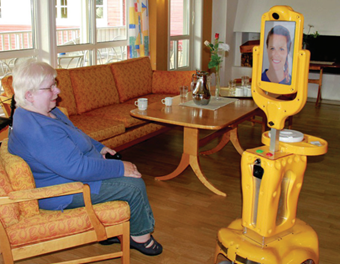
\includegraphics[scale=0.5]{P1.png}
\end{figure}
Design Review Report 3\\\  Telepresence Robot for Elderly \\\ \\\ \\\ Sponsor: JI CFE as part of mHBR initiative \\\ Mentor: Prof. Pradeep Ray, Prof. Artur Serrano \\\ Instructor: Prof. Guo Yunlong }
\author{Pan Chongdan\qquad  \\Boaro Fernando\\Liu Niyiqiu\\Qiu Tianyu\\Zhou Ruixing}
\date{Date: \today}
\begin{document}
\maketitle
\newpage
\tableofcontents
\newpage
\section{Introduction}
\gadd{
\subsection{Project Motivation}
With the acceleration of life rhythm, people usually spend more time away from home, causing more loneliness for the elderly. Under the circumstances, caregivers will be worried about the elderly's well-being and the elderly may feel a loss of bond with family and children. Telepresence robot is designed to cope with such scenario because caregivers can communicate and provide care for the elderly with the robot when they're away. From emotion perspective, the telepresence can play a role as an substitute of the caregivers so that it can enhance the connection between the elderly and their children
The telepresence robot for elderly mainly aims at providing remote care for the elderly when their caregivers are far away from them. Indeed, the robot can play a row as an alternative of personal visits and provide a real network of care.

\subsection{Customer Requirement}
Nowadays, there are telepresence robots products used in Europe now, and relative research shows they indeed increased feelings of happiness, self-esteem and reduced levels of frustration of their users.However, they're extremely expensive and hard to operate because a lot of limitations like unstable network communication caused by firewall.} We still need to solve some problems of current products.
\gadd{
\subsubsection{Problem}
\begin{enumerate}[1]
\item \textbf{Budget}
\par Our budget is under 1000 dollars while the products in the market is much more expensive than that, which implies that it will take much money to relative the robot's functions. The biggest problem for us is to redesign, simplify the robot and realize the essential functions without spending a lot of money.
\item \textbf{Telepresence Technology}
\par The core technology of telepresence robot is to establish stable and simple connection between the controller and the robot. Since firewall and routers are often used, there are many obstacles impeding the transmission of control signal. What's more, since the caregivers will keep moving, so the mobility of such control system is very important.
\item \textbf{Stable Control System} 
\par To realize available control between the caregivers and the robot, core processor, actors and sensors are essential. First we need to control actuators by giving instructions to the core processor connected the network. Then feedbacks will be given by sensors so that the caregivers can know the status of the robot. One of the most important task for our team is to create a available interface between the robot and caregivers so that they can control it smoothly.
\item \textbf{Functions for the elderly}
\par It's important to realize functions specially for the elderly. Since the elderly usually have different needs and different characteristics, the robot should be able to cope with different kinds of people. For example. different old people have different pills to eat at different time, so the medicine dispenser should be flexible enough to coordinate with it. It should be able to dispense various pills at once.
\item \textbf{Safety and Power}
\par Since usually the elderly usually stay with the robot alone, safety is very important and the nominal voltage shouldn't be too high, which is less than 30V. In addition, the robot should has a battery of high capacity so that it doesn't need frequent charging because it's hard for the elderly to bow and deal with the power supply.
\end{enumerate}}
Therefore, the customer requirement for our project is set based on main problems of the current product.
\begin{enumerate}[-]
\item The robot should be simple and cheap enough, which costs less than 1000 dollars but still keeps its essential functions.
\item Caregivers can have full control of the robot even when he is very far away from it. The remote control system should only have short lags and be free from firewall interruption. When caregivers drive the robot remotely, there should be a navigation system for him so that he can view the surrounding situation. The robot structure should be very stable to avoid trumbling.
\item Caregivers and the elderly can use this robot to make video and audio call to each other with acceptable lags and clarity. They should able to see each other's face clearly and hear what they say through the robot.
\item Caregivers can control the robot to give pills to elderly with a stable dispenser. The robot should be able to store the pills for a long time when caregivers is away and the pills won't go bad.
\item Different customers can make minor change to the robot for individual customization.
\end{enumerate}
\gadd{
\subsection{Competitive and Related Products or Technology}
\subsubsection{Giraffe Telepresence Robot}
All the similar products in market right now is much more expensive than 1000 dollars, and the most representative product is \textbf{Giraffe} produced by a Europe company.
\begin{figure}[H]
\centering
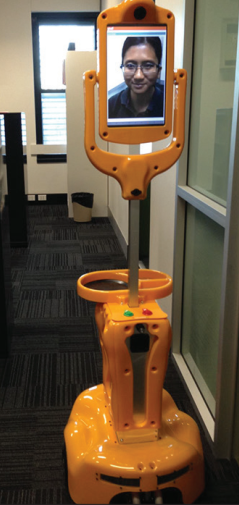
\includegraphics[scale=1]{P2.png}
\end{figure}
Giraffe has been put into the market for some time and it does have an effect on providing care and emotional connection to the elderly. However, it still have some problems such as firewall issues, video freezing, and driving lag etc, but it can be a reference based on which we can design and build our own telepresence robot.
\par In China, there is no such robot products but some smart furniture can be our competitive products.
\subsection{Relevant Hardware \& Software}
\subsubsection{Raspberry Pi}
\begin{figure}[H]
\centering

\includegraphics[scale=0.15]{P3.png}
\end{figure}
Raspberry Pi is a micro computer with many I/O interface so that it's easy for us to develop and control functions based on it. In addition. sin raspberry has its own linux system, we can write some control codes and realize Internet connection through it. Raspberry Pi can be a good central core for the telepresence robot.
\subsubsection{Team Viewer}
\begin{figure}[H]
\centering
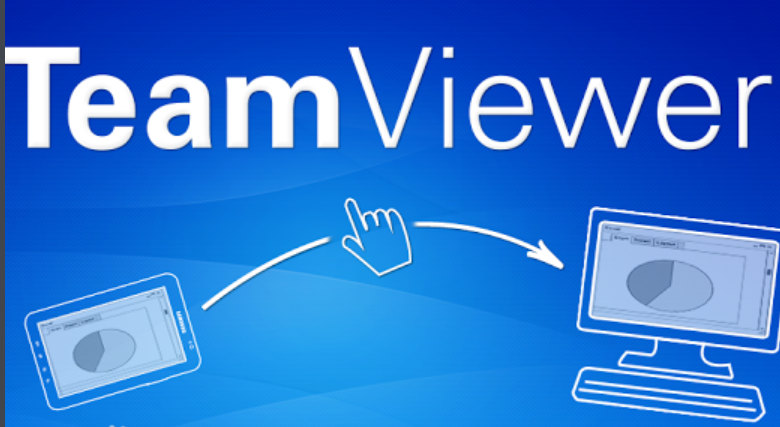
\includegraphics[scale=0.3]{P4.png}
\end{figure}
Team Viewer is a software developed by Germany which can provide stable remote control between different computers. What's more team viewer can be applied on any devices connected to world wide web as long as it has its own operating system. Team viewer is an important technology to realize stable remote control and control mobility of telepresence
\subsubsection{Screen, Camera and other Actuators and Sensors}
There is big screen which can be connected to the raspberry pi. With such screen, the elderly can communicate with the caregivers visually and freely. On the other hand, camera like opencv can get pictures from the elderly or the surrounding environment for the caregivers so that they can control the robot and contact the elderly more easily. Actuators and sensors will play an auxiliary role for realize such functions.
}
\section{Engineering Specification}
\gadd{
\subsection{Information Sources}
\subsubsection{Medicine Dispenser}
\paragraph{Background}
More than 50\% of the older people are living with multiple chronic illnesses\cite{2}. Thus, routine monitoring and assessment of the individual’s adherence is crucial to improve their health outcomes. Elderly with multiple chronic conditions face the complex task of medication management that can involving multiple medications of varying doses at different times. Advances in tele-health technologies have resulted in home-based devices for medication management and health monitoring for the elderly\cite{3}. The function of such medication dispensers is to alert the patient when it is the date and time to take their prescribed medication\cite{4}. When the time comes to take the medication, the pill dispenser automatically releases a pre-measured dose for consumption.
\paragraph{Medicine Dispenser Standards\cite{5}}
\begin{itemize}
    \item Provides audible, visible or vibration alerts.
    \item Dispenser must be locked once medicine is replenished.
    \item Long distance connectivity to track use.
    \item Humidity resistant and tamper proof.
    \item Dispense only the prescribed amount at the required times.
\end{itemize}
\subsubsection{Telepresence Robot}
\paragraph{Telepresence Robot Standards}
Telepresence Robots are a very new and unique type of robot in the market nowadays, and since there are standards for collaborative industrial robots (Cobots) and AGVs (automated guided vehicles) our robot would not be included in such standards because 1) Our robot does not include a robotic arm so it is not considered an collaborative industrial robot and 2) Since our telepresence robot will be a simplified version of our competitors due to our budget restriction, we will not be adding any obstacle avoidance sensors, instead, the person controlling the robot is responsible for its movement, thus it cannot be considered and neither can AGVs. The standards we have to abide by will therefore be our electronic components such as battery and CPU, but since we will buy our batteries and CPU from third party manufacturers (already passed safety regulations and standards) we will not have to worry about any hazard as long as we use the equipment correctly according to the manufacturers.
\subsection{Engineering Specifications}
The custom requirements of our project are divided into the software and hardware part. They are summarized as follows:
\subsubsection{Hardware Standard}
\begin{enumerate}
	\item The screen, along with its control buttons, should be large enough 
	\item The speaker should be loud enough for the elderly 
	\item The height of the screen should be suitable for old people who sit in a chair to watch 
	\item The medicine dispenser should be located on a suitable height 
	\item The medicine dispenser should have large storage 
	\item The medicine dispenser should provide dry environment to store the medicines
	\item The moving speed of the chassis should not be too fast or too slow
	\item The battery duration of the robot should last a long time 
	\item The physical entity of the robot does not contain any sharp edges 
\end{enumerate}
\subsection{Software Standard}
\begin{enumerate}
	\item Control (both local and remote) of the robot should be easy 
	\item Has alarm function to remind the elderly to take medicines
	\item Has auto obstacle detection and evasion algorithm 
\end{enumerate}

Besides these requirements from the two aforementioned categories, the total cost of the robot should be below 1000\$.

Considering the robot itself, we separate the robot into the following four functional parts: 1) Chassis of the robot, 2) Medicine Dispenser, 3) Touchscreen \& camera, 4) Raspberry Pi controller. The generated engineering specifications, along with the custom requirements are shown in Fig.~\ref{fig::qfd}.}

\begin{figure}[H]
	
	\centering
	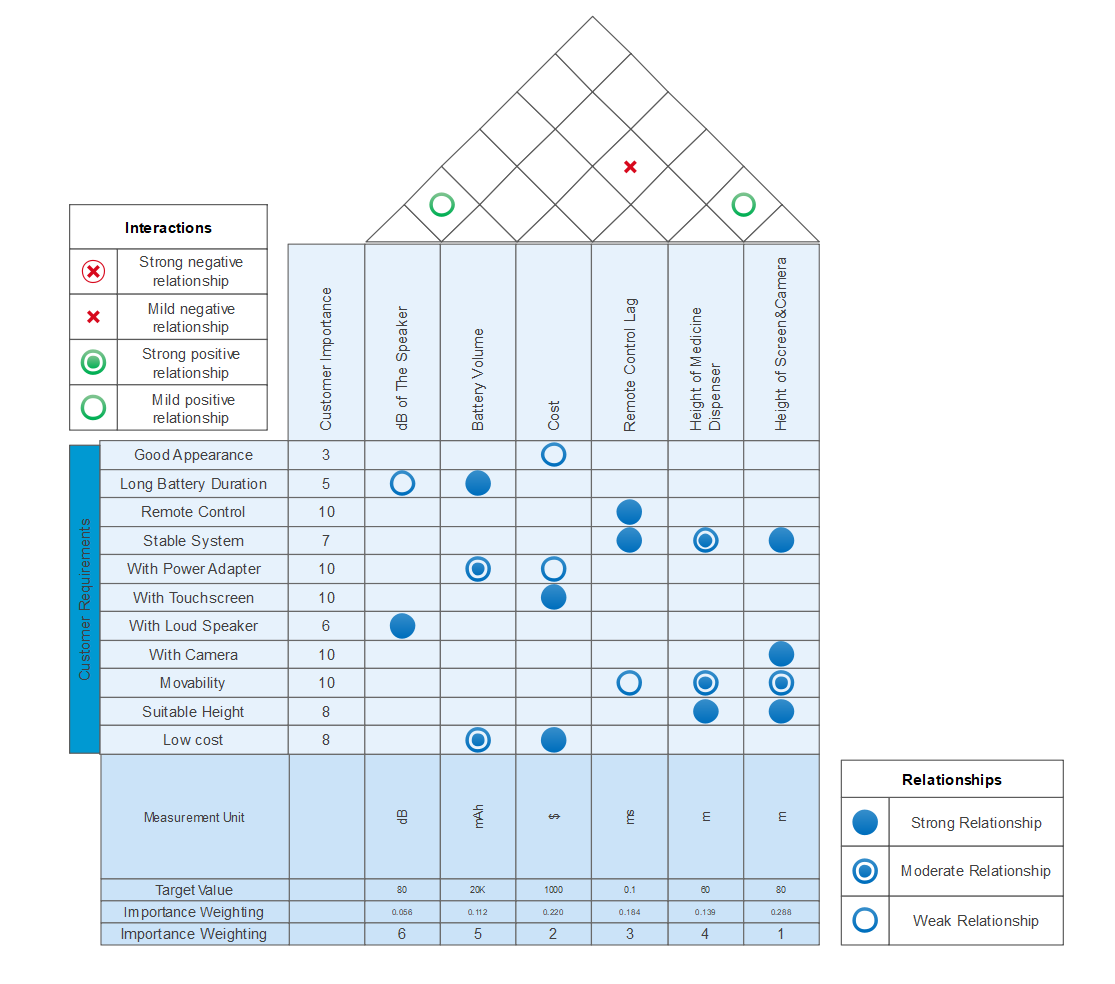
\includegraphics[width=5in]{Z5}
	\caption{QFD table of our project.}
	\label{fig::qfd}

\end{figure}
   In Fig.~\ref{fig::qfd} above, we list 12 customer requirements and 10 engineering specifications, rate their relationships, and calculate the priority. Each strong relationship counts 9 points, each moderate relationship counts 3, and each weak relationship counts 1. Multiply by the importance points of the requirements, we can calculate the weighted average of each specification. The specification with highest weight has the highest priority. We found out that the remote control lag is the most important one, and the motor power and the weight follow. The least important one is the dB of the speaker. Tab.~\ref{tab:spec} shows the details of the specifications.
\section{Selected Concept Description}
\subsection{Chassis}
Considering the end user of our product, the design of chassis requires a lot of considerations as well. First of all, it should be stable enough to support a one-meter-long aluminum rod with a bunch of components installed on it. It should have a particular trafficability such that it can move freely in narrow places at home. Also, it should have enough space to plant electrical components and batteries, and cover them well so that no dangerous components are outside to hurt the elders. Finally, it should look well, give the users a good impression.
\subsubsection{Version I}
The first version of the chassis has come up at the very beginning of this project. Since the upper part of the robot had not been designed, the chassis was made as general as possible. It consists simply two round acrylic boards, with an array of holes for further assembling. It’s only for temporary use, so the details are not put into consideration.
\begin{figure}[H]
	\centering
	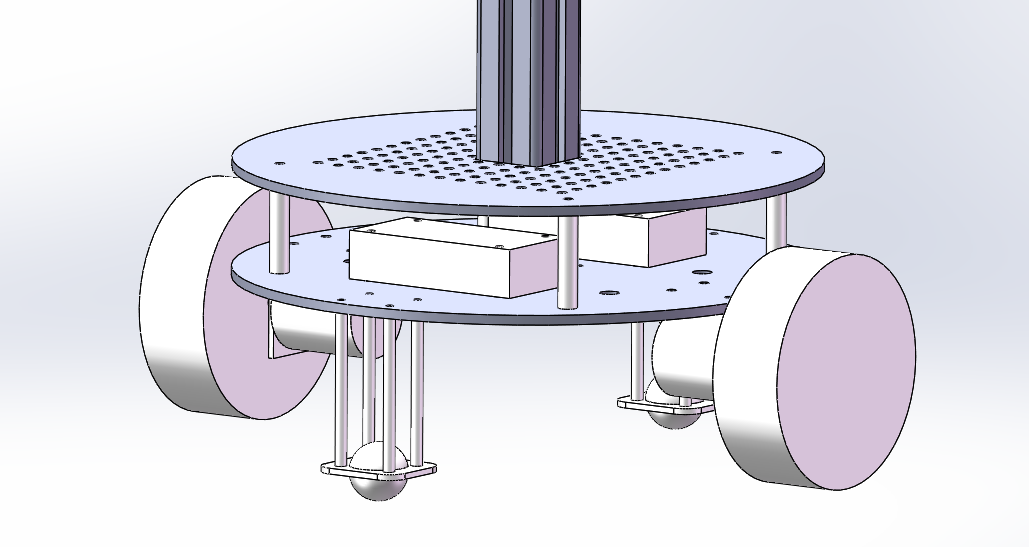
\includegraphics[width=0.7\linewidth]{Z1}
\end{figure}
\subsubsection{Version II}
The new version was updated basing on the use experience of the old one. In the new design, we fixed the existing problems. First of all, our team found out the old one is not stable enough. Because of the usage of universal wheel, the whole robot would wobble while we control it to turn. Therefore, we lowered the chassis, and used a universal ball instead. Also, to increase the stability, we change the shape of the acrylic boards from a round into a circumscribed square of it, which increases the space to set the electrical components at the same time, while the trafficability is not changed (since the width are the same.) Another improvement is the assembling method of the aluminum rod. In the old version, there was no consideration on how to assemble the rod onto the chassis, so what we did was fixing an aluminum cross on it and screwing the rod on the cross. It was not only ugly, but also dangerous, since there were too much sharp edges exposed outsides. In the new version, we make one square hole for the rod, so it can stick inside. For the same reason, we hide the wheels inside the chassis, so it is well-packaged.
\begin{figure}[H]
	\centering
	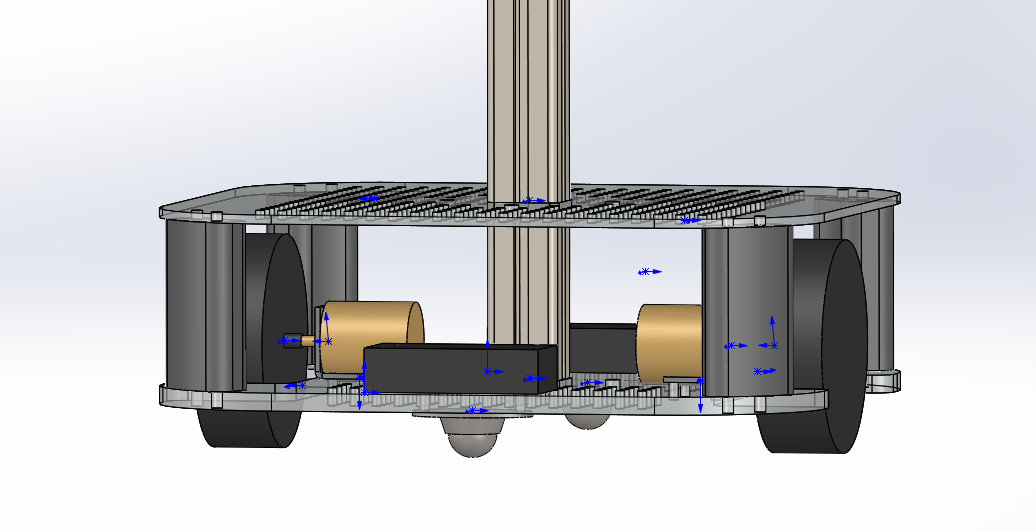
\includegraphics[width=0.7\linewidth]{Z2}
\end{figure}
\subsubsection{Overview of Selected Concept}
The final chassis we use is shown in fig. XI. As we can see, all the components are set between the upper and lower boards, therefore, it’s both stable and safe. We use the universal balls at the front and the back, so that the weight center of the robot will not change during turning process. The driving wheels are directly connected to the motors, which are controlled by a raspberry pi just near them. Aside of them, are batteries supplying power for both chassis and upper components. Also, a square hole is prepared for the aluminum rod, so that the connection between chassis and upper components are stable.
\begin{figure}[H]
	\centering
	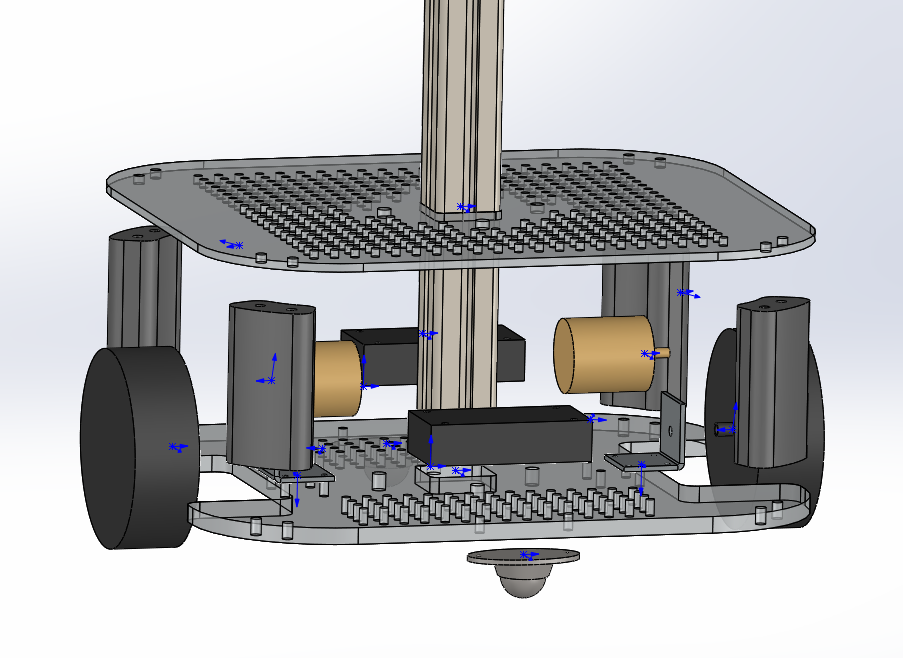
\includegraphics[width=0.7\linewidth]{Z3}
\end{figure}
\subsection{Medicine Dispenser}
For our medicine dispenser concepts we had to keep in mind our budget restraints, our end user, and the safety standards. Which meant that the design had to operate with few electrical components (motors, servos, etc..), to be simple enough to cheaply 3D print, to be easily handled by the elderly and their caregivers and to comply with the safety standards (mainly correct dosages, tamper proof and humidity proof).
\par The two concepts that were generated were based on the way that the pills would be sorted and delivered to our users. In the first concept the daily medication would have to be sorted by the caregiver and the cocktail of medication would have to be put into each slot manually. The second concept would have blocks in which each block would contain one type of medication, and the system would separate them automatically depending on the demand.
\subsubsection{Mixed Pill Manual Sorting}
\begin{figure}[H]
	\centering
	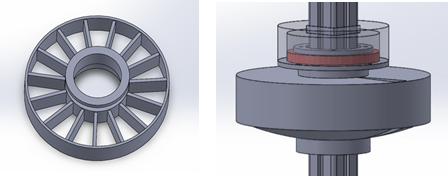
\includegraphics[width=0.7\linewidth]{M1}
	\caption{Mixed Pill Manual Sorting Design}
\end{figure}
The main idea for the first concept was to have the caregiver sort a days’ worth of medication and load them into each slot in the dispenser, the dispenser would then rotate at the desired time so that the medication that was in the next slot would fall into a tray and be consumed by the user.
\subsubsection{Pill Blocks Automatic Sorting}
\begin{figure}[H]
	\centering
	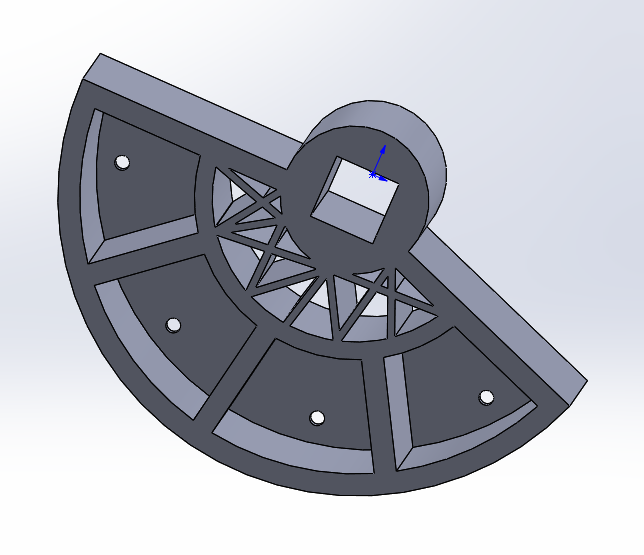
\includegraphics[width=0.5\linewidth]{M2.png}
	\caption{Pill Blocks Automatic Sorting Design}
\end{figure}
For the Pill Blocks concept the main idea was to have the caregiver load the blocks with the same type of pill, and the system would dispense into a tray the desired amount of each pill at the designated time. Each block would have its own mechanism to make sure that only a single pill would be released at a time, so that the user would have the correct dosage of medication.
\subsubsection{Concept Selection Process}
With both our medicine dispenser designs, the Mixed Pill Manual Sorting and the Pill Blocks Automatic Sorting being plausible choices for our needs, we will construct a scoring matrix in order to compare them with our requirements (price, user and safety) in order to ensure the best results. We will also go into more detail about each design’s strongest and weakest points, and whether they outweigh our decision.
\begin{figure}[H]
	\centering
	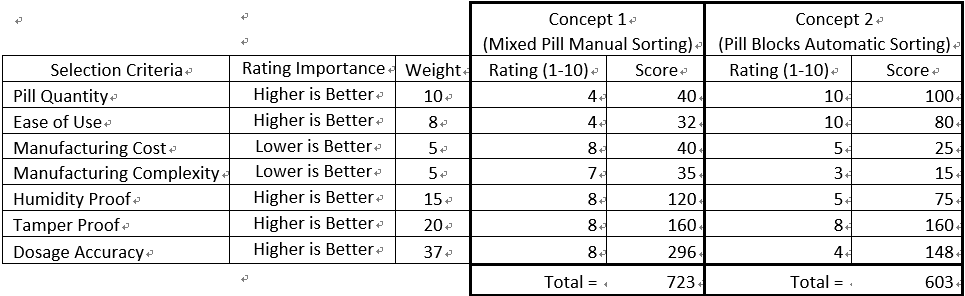
\includegraphics[width=0.75\linewidth]{M3.jpg}
\end{figure}
We can see from the criteria and the weights that the safety aspects of our medicine dispenser outweigh the usability and cost. Therefore since our Mixed Pill Manual Sorting concept has a higher score we have chosen to pursue this design.
\par The main benefit of Concept 1 (Mixed Pill Manual Sorting) is its simplicity and reliability, there is very little room for error since the caregiver is sorting the medicine dosages and the mechanism safely stores them until the predetermined time in which the dosage is dispensed using an accurate stepper motor which always knows it’s current position in the 360o movement. And this reliability is crucial when leading with something as important as someone’s medication. Its weak point would be the refilling of medication, where the caregiver would have to manually sort the medication and insert each cocktail into the separate compartments, making it less user friendly.
\par For our second concept (Pill Blocks Automatic Sorting) the main benefit would be its autonomous sorting, where the caregiver would only have to pour the pills into each block and not have to sort them. The biggest downfall with the design also comes from this autonomous feature, since it is very hard to sort medication of different sizes, colors and textures, it makes the dosage accuracy (most important criteria) low. In order to ensure correct dosage, we would have to have a mechanism in each block that only lets one pill through at a time (which is very hard for different pills) and a checking system to make sure that there aren’t two pills or no pills being dispensed, because an over dosage or under dosage could cause serious repercussions. Therefore an automatic sorting mechanism would be overly complicated and expensive to manufacture with our required safety specifications.
\subsubsection{Overview of Selected Concept}
\begin{figure}[H]
	\centering
	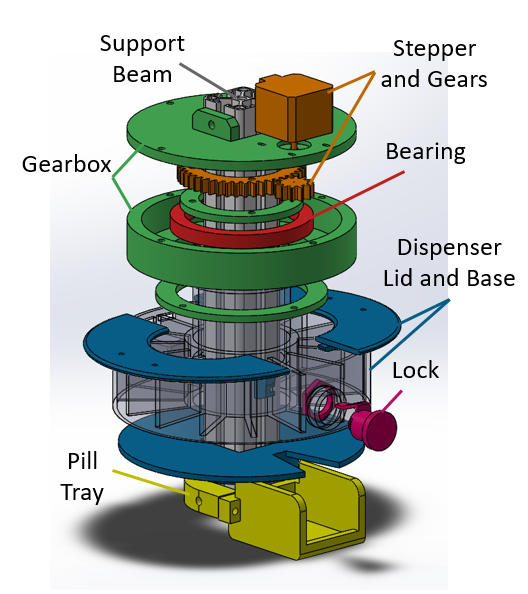
\includegraphics[width=0.3\linewidth]{M4.png}
	\caption{Exploded View of Medicine Dispenser}
\end{figure}
Our chosen concept has five sections as we can see in Fig. 4. The stepper motor, gears and bearing (orange and red) are responsible for the movement of the dispenser base. The support beam (silver) is connected to our chassis, and it supports the gearbox, bottom dispenser base and the pill tray which are all fixed to it. The gearbox (green) houses the moving parts so they are safely away from the users as well as keeps the dispenser suspended and rotating freely with the bearing. The dispenser lid and base (blue and transparent) house the pill boxes and keep them humidity proof. The lock (pink) locks the dispenser lid in place so that once the pill boxes are inside the dispenser they are tamper proof. And finally the pill tray (yellow) receives the pill boxes once they drop from the dispenser, making it easy for the user to administer the drugs.
\subsubsection{Engineering Design Analysis}
\paragraph{Medicine Dispenser}
\par Our first design iteration started with the barebones of the system:
\begin{enumerate}
\item Dispenser frame which would house the pills.
\item Bottom dispenser which would only allow one dosage to be administered per time.
\item Pill tray for easy access to the medicine.
\item Gearbox for our bearing and gears.
\end{enumerate}
\begin{figure}[H]
	\centering
	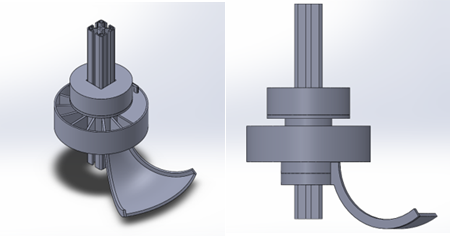
\includegraphics[width=0.75\linewidth]{M5.jpg}
	\caption{First Iteration of Medicine Dispenser Design}
\end{figure}
\par Dispenser frame: our initial design was built with 31 partitions for one month use of dosages, but the pills were to be directly deposited into each partition; this was a problem because the pills would move with the dispenser frame while they scrapped against the bottom dispenser which is fixed. This design would both cause damage towards the pills as well as make it hard for us to block humidity out of the system. There was also a clearance problem between the gearbox and the dispenser frame which was too short to comfortably deposit the pills into their partitions. The last issue with our frame was the lack of a locking mechanism to keep the pills tamper proof. Our solution to these problems was to decrease the number of partitions to 15 for two weeks of use, making each partition big enough to fit a pill box, which would simultaneously keep the pills humidity proof and prevent them from scratching against the bottom dispenser, for the clearance problem we elongated the frames connection to the bearing by 50mm which allowed comfortable user experience, and finally we adapted the frame to include a two point of contact lid and a hole for the lock in one of the 15 partitions.
\par \textbf{Bottom Dispenser} the first design of the bottom dispenser was a curved half sphere shape so that the pills would be able to slide toward the center closer to the support beam, and be able to slide easier when reaching the pill tray, but this design was quickly modified due to the difficulty of 3D printing and the introduction of our pill box.
\par \textbf{Pill Tray} in order to make it easier for the users to access their medication, a pill dispenser was designed with a slide shape to ensure the safety of the medication once it was dropped from the dispenser. The slide design was modified because of the difficulty to 3D print the design as well as the change from individual pills to the pill box, which would mean the tray would have to “catch” a little box full of pills instead of multiple individual pills.
\par \textbf{Gearbox} our gearbox for the first design iteration was very incomplete, with only the bearing and frame fixture being designed, it was one of the sections that most needed development once the concept was chosen. For the second iteration of the design the gearbox was modified to be run by a servo motor that was connected to two helical gears, which would turn the dispenser frame. The power input for the gearbox was another item that needed multiple iterations. Since our servo motor could not be controlled with our required accuracy. We switched to a small stepper motor, which was able to control our dispenser accurately (the gears were also designed so that 48 steps would equal one iteration), but only when it was empty, for the added friction of the pill boxes would change the number of steps for each iteration. So lastly we designed the gearbox to be run by a stronger and more accurate stepper motor (400 steps per iteration), which fulfilled all our needs of accuracy and power. The three designs of the gearbox lid can be seen in Fig.5 below.
\begin{figure}[H]
	\centering
	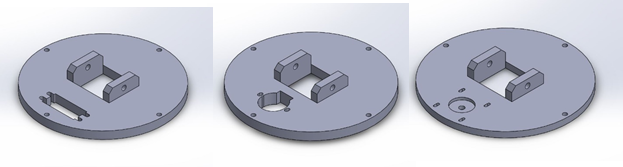
\includegraphics[width=0.75\linewidth]{M6.jpg}
	\caption{Gearbox Lids for Servo, Small Stepper and Large Stepper Motors}
\end{figure}
\par In our completed design iteration in Fig. 6 below we can see that all the necessary components are designed and bought (bearing, stepper motor and lock) or 3D printed (gearbox, gears, dispenser and pill tray) to meet our engineering specifications and requirements.
\begin{figure}[H]
	\centering
	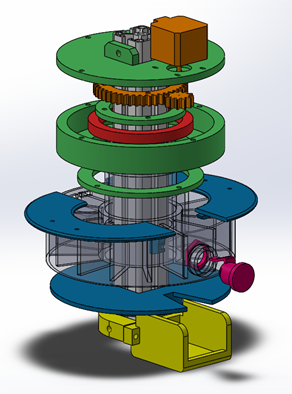
\includegraphics[width=0.5\linewidth]{M7.jpg}
	\caption{Completed Design of Medicine Dispenser}
\end{figure}
\subsubsection{Design Description}
In our bill of materials Fig. 7(3.3) below we can see the 18 parts that compose our medicine dispenser. All parts are 3D printed except for the bearing (item 6 in Fig.7.3.3), the stepper motor (item 4 in Fig.7.3.3) and the lock (items 14 and 15 in Fig.Fig.7.3.3) which were purchased. The whole assembly (without aluminum extrusion) measures in 220mm tall and 192mm x 180mm wide. The individual parts and their dimensions can be found in Appendix I. The working principal of the system starts from the stepper motor (item 4 in Fig.Fig.7.3.3), which is fixed to the small gear (item 12 in Fig.7.3.3) which in turn rotates the bigger gear (item 11 in Fig.Fig.7.3.3). The bigger gear is fixed to the top dispenser (item 2 in Fig.7.3.3), and when it rotates the programmed steps it will drop the pill box (item 13 in Fig.7.3.3) onto the pill tray (item 17 in Fig.7.3.3). From there the user has access to their pill dosage.
\begin{figure}[H]
	\centering
	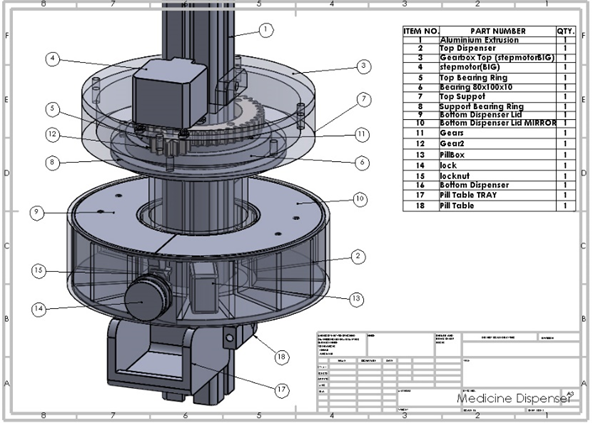
\includegraphics[width=0.7\linewidth]{M8.png}
	\caption{Medicine Dispenser Bill of Materials }
\end{figure}
\subsection{Software Implementation}
From the software side, the engineering specifications and custom requirements of our design indicates implementation in the following three areas:
\begin{enumerate}
	\item The control system which control the movement of the chassis
	\item The communication system that allows remote control of the robot
	\item The video streaming system
\end{enumerate}
\begin{figure}[H]
	\centering
	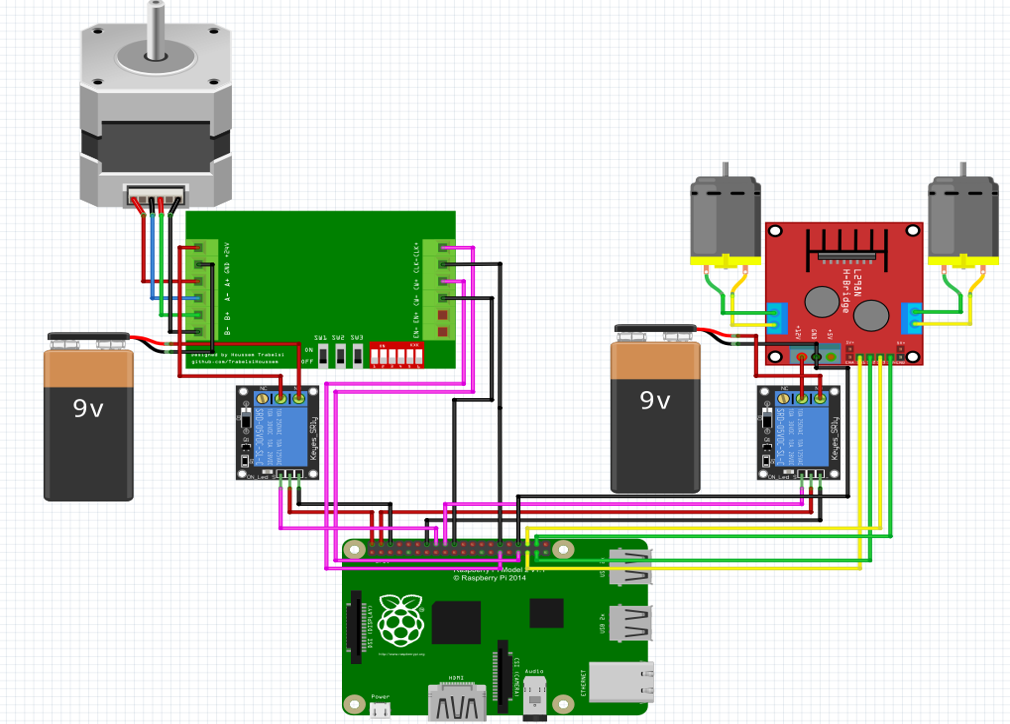
\includegraphics[width=0.7\linewidth]{circuit}
	\caption{The circuit in the chassis part of the robot. }
	\label{fig:circuit}
\end{figure}

\subsubsection{Control System}
The raspberry pi board contains a set of general purposed input output (GPIO) pins. Through these IO pins, we are able to control the movement of the robot. The physical circuit is shown in Fig.~\ref{fig:circuit}. The control program is shown below.
\begin{lstlisting}[language=python]
#!/usr/bin/env python3
# -*- coding:utf-8 -*-
from bottle import get, post, run, request, template

import RPi.GPIO as GPIO
import time

#left wheel motor
LeftM1 = 35
LeftM2 = 37

#right wheel motor
RightM1 = 36
RightM2 = 38

#stepper pin
StepperStep = 33
StepperDir = 29
OldStepper = [13, 15, 16, 18]



def setUp():
	GPIO.setmode(GPIO.BOARD)
	GPIO.setwarnings(False)
	GPIO.setup(LeftM1, GPIO.OUT)
	GPIO.setup(LeftM2, GPIO.OUT)
	GPIO.setup(RightM1, GPIO.OUT)
	GPIO.setup(RightM2, GPIO.OUT)
	GPIO.setup(StepperStep, GPIO.OUT)
	GPIO.setup(StepperDir, GPIO.OUT)
	for pin in OldStepper:
		GPIO.setup(pin, GPIO.OUT)



def forward():
	GPIO.output(LeftM1, GPIO.HIGH)
	GPIO.output(LeftM2, GPIO.LOW)
	GPIO.output(RightM1, GPIO.HIGH)
	GPIO.output(RightM2, GPIO.LOW)

def backward():
	GPIO.output(LeftM2, GPIO.HIGH)
	GPIO.output(LeftM1, GPIO.LOW)
	GPIO.output(RightM2, GPIO.HIGH)
	GPIO.output(RightM1, GPIO.LOW)

def turnLeft():
	GPIO.output(LeftM2, GPIO.HIGH)
	GPIO.output(LeftM1, GPIO.LOW)
	GPIO.output(RightM1, GPIO.HIGH)
	GPIO.output(RightM2, GPIO.LOW)

def turnRight():
	GPIO.output(LeftM1, GPIO.HIGH)
	GPIO.output(LeftM2, GPIO.LOW)
	GPIO.output(RightM2, GPIO.HIGH)
	GPIO.output(RightM1, GPIO.LOW)

def stop():
	GPIO.output(LeftM1, GPIO.LOW)
	GPIO.output(LeftM2, GPIO.LOW)
	GPIO.output(RightM2, GPIO.LOW)
	GPIO.output(RightM1, GPIO.LOW)
	GPIO.output(StepperStep, GPIO.LOW)
	GPIO.output(StepperDir, GPIO.LOW)


def stepperForward():
	GPIO.output(StepperDir, GPIO.HIGH)
	for i in range(0, 48):
		GPIO.output(StepperStep, GPIO.HIGH)
		time.sleep(0.001)
		GPIO.output(StepperStep, GPIO.LOW)
		time.sleep(0.001)
	time.sleep(0.5)


def stepperBackward():
	for i in range(0, 128):
		highpin = i % 4
			for pin in OldStepper:
				GPIO.output(pin, GPIO.HIGH)
				time.sleep(0.003)
				GPIO.output(pin, GPIO.LOW)
				time.sleep(0.5)


def main(status):
	setUp()

	if status == "front":
		forward()
	elif status == "leftFront":
		turnRight()
	elif status == "rightFront":
		turnLeft()
	elif status == "rear":
		backward()
	elif status == "stop":
		stop()
	elif status == "leftRear":
		stepperForward()
	elif status == "rightRear":
		stepperBackward()


@get("/")
def control():
	return template("control")


@post("/cmd")
def cmd():
	adss = request.body.read().decode()
	print("The key pressed is: " + adss)
	main(adss)
	return "OK"


run(host="0.0.0.0")

\end{lstlisting}

In the first part of the code, the pins are defined. (See Line 7 to Line 19) The initialization of the pins are done in the function setUp. (See Line 24 to 33) The following functions forward, backward, turnLeft, turnRight, and stop (see Line 37 to Line 67) is the movement control function for the chassis. As is shown in Fig.~\ref{fig:circuit}, the chassis is controlled by two DC motor using L298 board. To start these motors we can simply output high voltage to the corresponding pins.

The control of the stepper motor, on the other hand, is more complicated (See Line 70 to Line 87). Here we implement Pulse Width Modulation (PWM) to control the precise angle for the motor to rotate. The two function stepperForward and stepperBackward are designed to make the motor rotate clockwise and counter-clockwise respectively. However, here we wrote the implementation of PWM for two different type of steppers for test purpose. In this report, the PMW control of the new stepper motor will be explained, which is implemented in the function stepperForward.

First we need to calculated the total number of steps that the stepper motor needs to perform for the medicine dispenser to rotate one block. The stepper motor drive the smaller gear, which has 12 teeth. The small gear is connected to the larger gear with 43 teeth. The larger gear drives the medicine dispenser. We have 15 blocks for the medicine dispenser. Therefore, the number of teeth rotated for the larger gear if the medicine dispenser rotates one block is calculated as
\begin{align*}
\text{Number of teeth rotated } = 43 / 15 = 2.867 \text{ teeth}
\end{align*}
The smaller gear also needs to rotate 2.867, which corresponds to $2.867/12 = 0.2389 $ round. The stepper motor we uses need 200 steps to complete a full circle. Therefore the number of steps needed for the stepper motor if the medicine dispenser rotates for one block is
\begin{align*}
\text{Number of steppers needed } = 0.2389 \cdot 200 = 47.78 \text{ steps}
\end{align*}
We round this value to 48. And this is the range for the loop shown in Line 72. The error of this rounding is calculated as
\begin{align*}
\varepsilon = \frac{48-47.78}{47.78} \cdot 100\% = 0.47 \%
\end{align*}
The above calculation shows how we calculated the number of steps needed. To implement the stepping process, we first initialize the direction pin of the stepper (See Line 71). Then we loop for 48 times and in each loop, we create a pulse by outputting high and low voltage alternatively (See Line 73 to 76).

The last part of the control program is the main function and the functions to realize the  listen utility provided by the bottle library in python. The main function set up all the pins and execute a function based on its input (See Line 90 to Line 106). Using decorators, we define two further functions to use the bottle library (See Line 109 to Line 119). The first function is used for request routing. The second function is used as event handler when user issued some control command via our web page interface. The detailed information of this user interface will be included on the next section. Last, we start a local server to listen to user commands (See Line 122).


\subsubsection{Communication System}
The graphic user interface of the control program is shown in Fig.~\ref{fig:gui}. The website coding and the script for the website is intuitive. Every time a button is pressed on the website, the website will post a "/cmd" request to the control program, which will then call the main function. The detailed description for the functions from the bottle library can be found through the website \url{https://bottlepy.org/.}

\begin{figure}[tbph!]
	\centering
	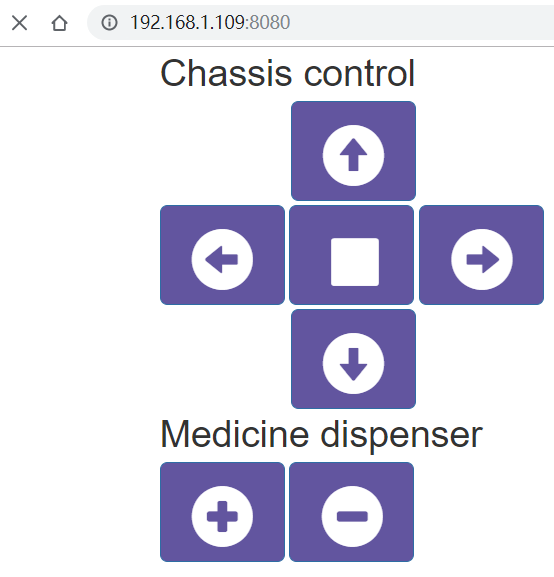
\includegraphics[width=0.5\linewidth]{gui}
	\caption{The web page of the control program}
	\label{fig:gui}
\end{figure}
In order to remotely log into the raspberry pi and the pad, we need a remote control system. We decide the use a developed software called TeamViewer to realize this function. The inclusion of TeamViewer aligns well with our custom requirement and engineer specifications because it supports multiple platforms and offers stable connection. Also, TeamViewer offers a private communication channel due to the 256 bit AES encryption scheme it adapts.
\subsubsection{Video Streaming System}
To realize video communication with the elderly and provide visual guide for remote control of the movement of the robot, we need a video streaming system to give real-time information to the user.
For this sub-system, we have tried two different implementations. The first approach is to write a streaming application by ourself. We bought a screen, a camera, and an audio output that is compatible with Raspberry Pi, as is shown in
Fig.~\ref{fig:screen}.

\begin{figure}[!htbp]

	\centering
	\subfigure[Screen]{
		\begin{minipage}[b]{0.3\linewidth}
			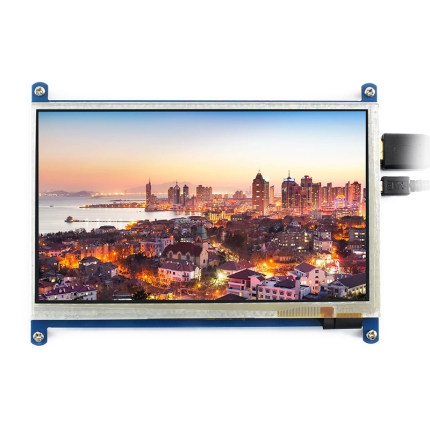
\includegraphics[width=1\linewidth]{screen}
		\end{minipage}
		\label{fig::non-disjunctive0}
	}
	\subfigure[Audio output]{
		\begin{minipage}[b]{0.3\linewidth}
			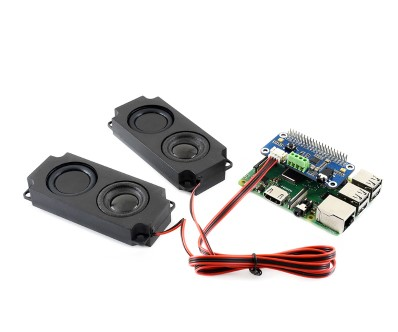
\includegraphics[width=1\linewidth]{audio}
		\end{minipage}
		\label{fig::non-disjunctive1}
	}
	\subfigure[Camera]{
		\begin{minipage}[b]{0.3\linewidth}
			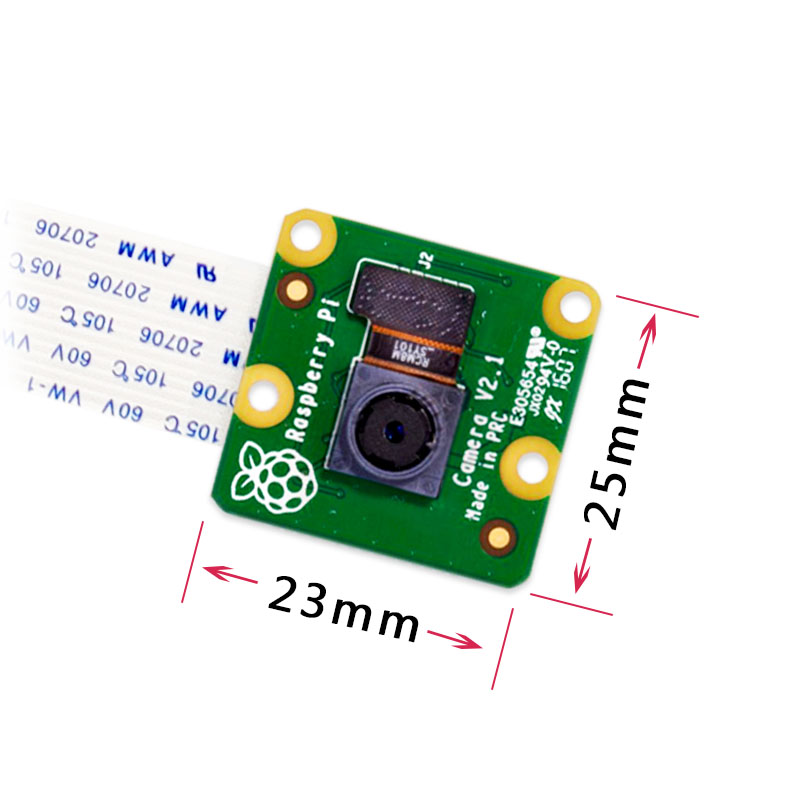
\includegraphics[width=1\linewidth]{camera}
		\end{minipage}
		\label{fig::non-disjunctive2}
	}


	\caption{The equipment initially used for the video streaming system}
	\label{fig:screen}
\end{figure}

We managed to realize the video streaming system using the application program interface (API) provided by v4l2 drive and displayed the camera view on the same web page as in Fig.~\ref{fig:gui}. However, we encountered the following problems
\begin{enumerate}
	\item We were only able to stream the camera view on Raspberry Pi to the web page. We also needed to stream from the user's device back to the screen.
	\item The streaming quality of our implementation was poor. There were sever video lags.
	\item We only streamed the video information. To realize the video communication system, we also needed to record sounds from both sides, output them to the corresponding devices, and performed synchronization with the video streaming.
\end{enumerate}

Solving these problems involves much programming in the hardware level, which is complicated and tedious. Meanwhile, we had only spent 1/5 of our budget. Therefore, we decided to buy a windows pad of which the video communication system is already implemented. With this pad, the video communication is very straightforward. We use apps such as WeChat or QQ to realize this function. Also, we can remote control the pad using TeamViewer.

\subsection{Manufacturing Plan}


\begin{table}[H]
	\centering
	\begin{tabular}{|c|c|c|c|}
		\hline
		Item& Quantity &  Price & Usage  \\
		\hline
		Raspberry Pi& 1 & 420  & Central processing unit  \\
		\hline
		Motors&  2&  87&   Basic movement\\
		\hline
		L298N drive board and wires& 1 & 100 &  Control motors\\
		\hline
		Arcylic board& N/A & 300 & Build chassis \\
		\hline
		Battery and charger&  1& 267 & Power supply  \\
		\hline
		Wheel &  2&  100& Basic movement \\
		\hline
		Windows 10 pad&  1& 1300 & Video call \\
		\hline
	\end{tabular}
	\caption{The list of components and materials needed.}
	\label{tab::material}
\end{table}

\par The list of materials and components needed to build the robot are listed in Tab.~\ref{tab::material}. To build the mechanical part of the robot, basic tools such as screw driver, file, hammar, saw, wrench, and electric soldering iron are needed. They are very common in a machine workshop. The assemble of all the components will take a team of 4-5 people approximately one day of time.
\par The acrylic boards of our chassis are designed by ourselves but manufactured by Taobao shop. The drawing of the upper and lower boards is shown below. The two motor and all wheels (including universal wheels and the driving wheels) are chosen and bought under the consideration of its specifications. The four pillars supporting the upper board were 3D printed, in order to match the shape and height, so that the out-look of the chassis would be smooth. Also, the aluminum rod should be connected with the upper board with four angles that were specially made for this rod, which were purchased along with it. 
\begin{figure}[H]
	\centering
	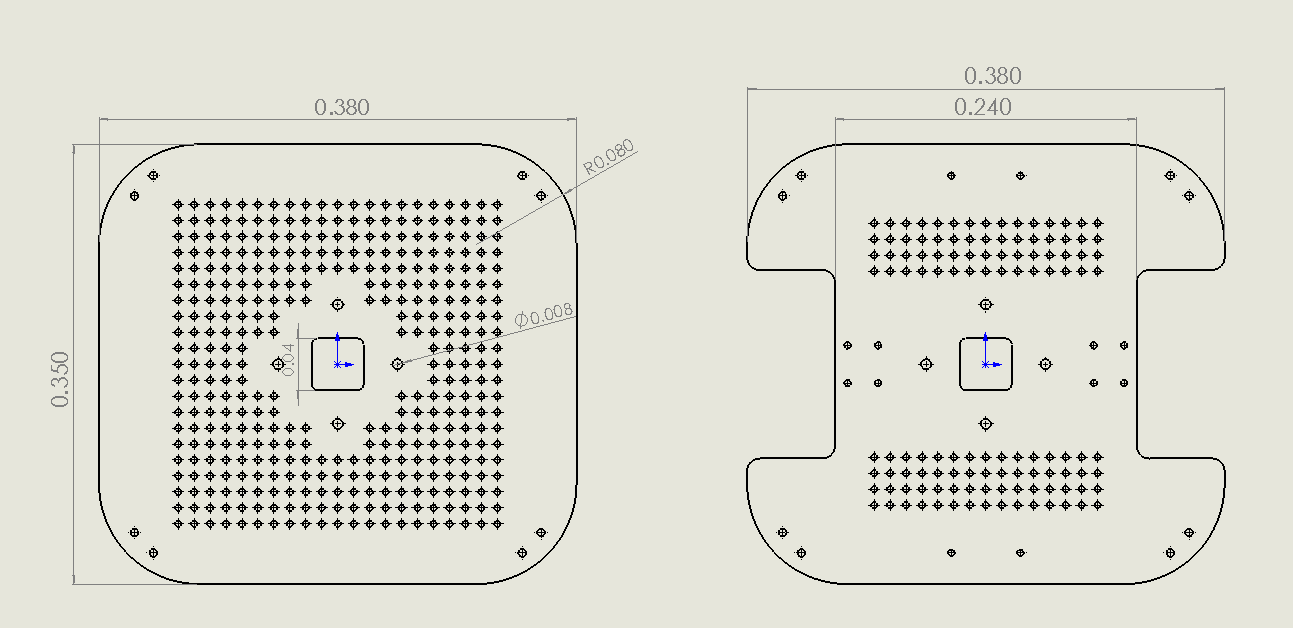
\includegraphics[width=0.7\linewidth]{Z4}
\end{figure}
\par In addition, most of our medicine dispenser parts/components (around 90\%) are 3D printed using a common PLA printer. The only parts that were bought were the bearing, the stepper motor and the lock, apart from the screws and bolts. Therefore the manufacturing process was mostly designing the dispenser to the correct dimensions to house the parts that were bought accordingly. We did design the 3D parts to fit tightly, so some filing of fittings had to be done to ensure a perfect fit. Our lock bolt was also slightly modified since it as too big for its intended location, we had to bend it, cut it and file it down, having our CAD drawing as a reference for angle and size.
\par Our tolerances are not very rigorous, as parts that have to come together tightly are designed with the same diameter and filed down for a perfect fit, while other parts that have to fit into one another easily are designed smaller to have no interference. The gearing is also designed so that the stepper motor can be moved 2mm forward or backwards to fit perfectly. So the more important tolerances would be in the holes, having them align and be of the correct dimension so that screws can be accurately inserted and secure the system. And less tolerance in the parts that fit in one another such as the dispenser lids and the bottom dispenser, since they work as intended even if manufactured with less tolerance.
\subsection{Validation Plan}
There are three major criteria to evaluate the quality of the product: the chassis movement, the medicine dispenser, and the remote video communication. Here we will present experimental set up to test their corresponding engineering specifications. For other engineering specifications such as the loudness of the speaker, the volume of the battery, the height of the screen, and the screen resolution, they can be directly measured or validated by reading the manual for each component used.
\subsubsection{Chassis movement}
To set up this experiment, a clear field is needed with a line of length 5 meters measured. The robot is placed at one end of the line. At the other end, a chair with person sit on it should be placed in a different direction with the robot. Through remote control, the robot should be able to forward in a straight line for the 5 meters, and then turn to the person. The user that control the robot cannot see the situation in the field directly. He or she can only move the robot using the view provided by the camera on the robot.

In this experiment, we will validate the moving speed of the robot and the video streaming specification.

\subsubsection{Medicine dispenser}

The experiment is set up in 10 rounds. In each round, we fill in the medicine dispenser with pills. Then we rotate the dispenser 14 times and see if the pills can be correctly dispensed. The number of failures are recorded. In each round, pills with different weights should be applied.

In this experiment, we will validate the functionality of the medicine dispenser, as is required by the engineering specification.


\subsubsection{Remove video communication}
To perform this experiment, we need another stable video communication tool as a reference. We turn on the video communication utility of the robot and the reference tool at the same time. Then a third person will shoot the video conference using a camera. By analyzing the time delay between the streaming of these two tools, we are able to get the delay of the video communication utility of the robot.

In this experiment, we will validate the engineering specification for the video communication lag.
\section{Project Timeline and Plan}
\gadd{
\subsection{Project Milestone \& Gantt Chart}
Three students major in ECE and two students major in ME form our group.
Considering team members’ specialties, our project is mainly divided into mechanical
part and software development and integration part.
\par The mechanical part concerns mostly the hardware of the robot. Fernando and Ruixing are mainly in charge of designing and building medicine dispenser,
fall detector and assembling and testing the robot.
\par We plan to build our first prototype before the end of October, then Pan Chongdan will communicate with our sponsors at Norway and get some feedback. In November, we will make adjustments to the robot according to the feedback.
\begin{figure}[H]
	\centering
	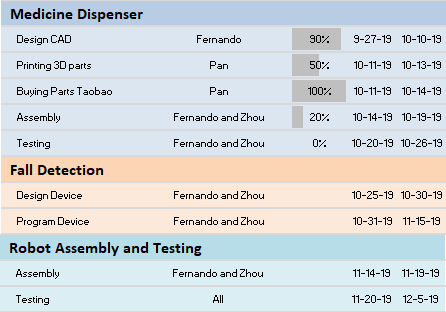
\includegraphics[width=0.75\linewidth]{ganttA.png}
	\caption{ME Gantt Chart}
\end{figure}

The software and integration part mainly consists of robot movement control,function implementation and user interface design. Chongdan and Niyiqiu
are mainly in charge of user interface design. Niyiqiu and Tianyu are in charge of function implementation, and Chongdan and Tianyu are in charge of the circuit design of the robot.
\begin{figure}[H]
	\centering
	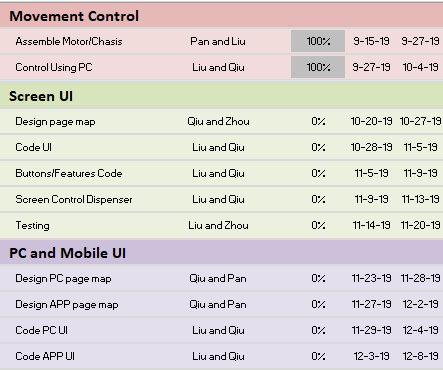
\includegraphics[width=0.75\linewidth]{ganttB}
	\caption{ECE Gantt Chart}
\end{figure}
From our complete Gantt chart. we can see the groups progress with
our tasks. We are prioritizing the robots functionality such as smooth movement,
medicine dispenser and fall detection, therefore these tasks are towards the earlier
weeks. While our user friendly interface although very important is left for the later
10weeks since it is not an integral part of the project. Our progress so far has been
acceptable, although we are a little behind schedule with the medicine dispenser,
movement control has been completed and we are satisfied with the results. We are
also getting ready to start work on our screen UI and fall detection tasks. We should
have no problem in being able to deliver a finished product with all its working
specifications by the end of the semester.
\begin{figure}[H]
	\centering
	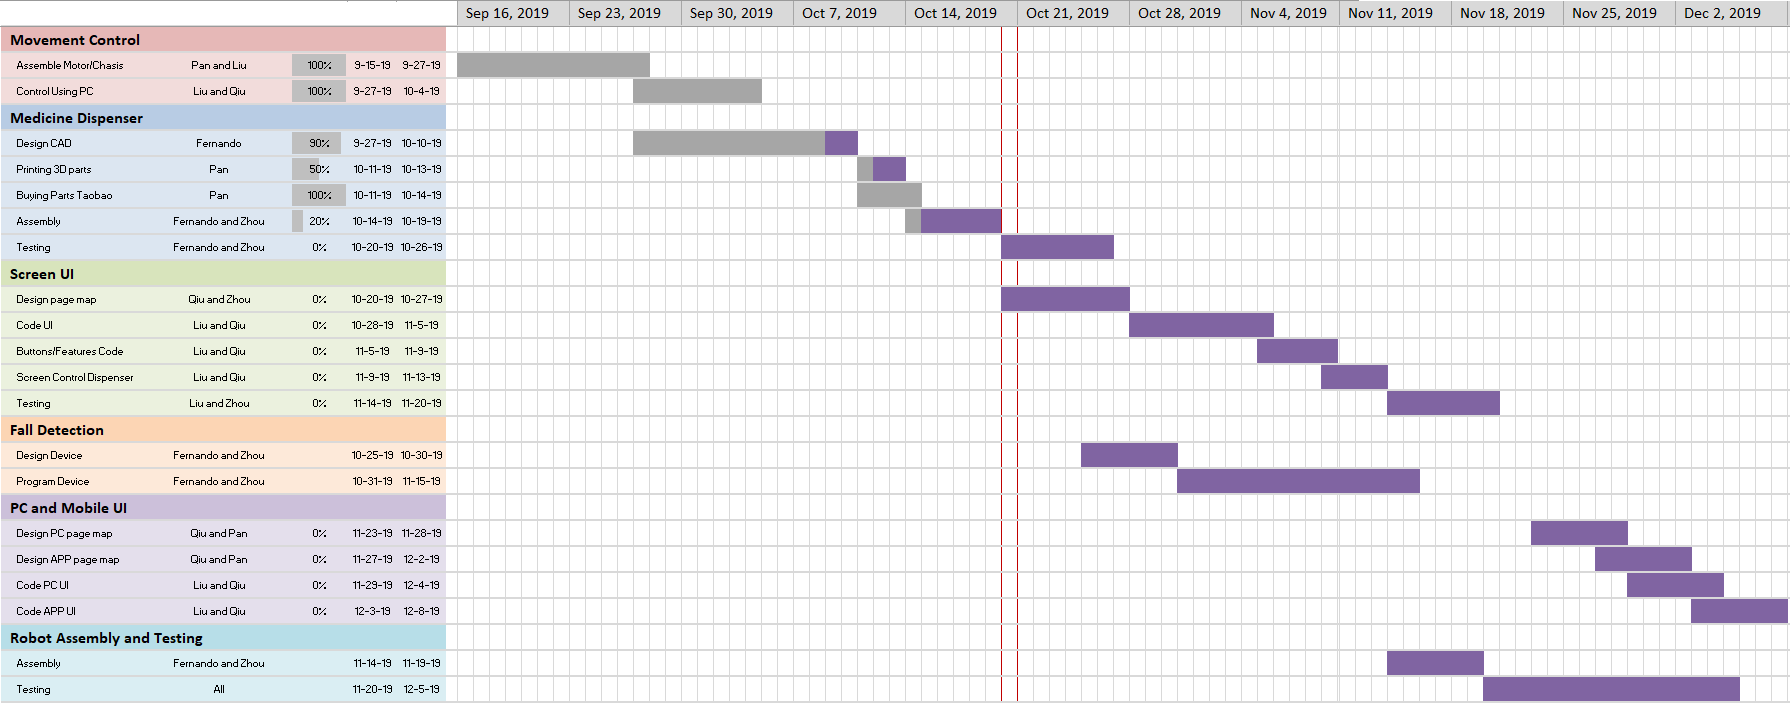
\includegraphics[width=0.8\linewidth]{ganttC}
	\caption{Gantt Chart}
\end{figure}
}
\par Up to now, our progress has been ahead of time. The medicine dispenser, the remote control system and movement control have all been validated. In the week from Nov.20 to Nov.27, the main work is the replacement of chassis and assembly the entire robot. In the following week, overall test will be conducted and all functions will be tested repeatedly to ensure feasibility and stability. The following Gantt Chart indicates the schedule of our project. The purple bars represent tasks that have already been done, while grey bars representing tasks left to be done.
\par In the next week before Design, there are still following improvements can be made:
\begin{enumerate}
\item Increase chassis stability. We are going to change the chassis plate with thicker ones, which will definitely more difficult to bend. Also the upper plate and the lower plate will be linked together by long screws to be kept parallel.
\item Add relays (switches) to DC motors for robot moving and stepper motors for medicine dispenser’s rotation. Since stepper motor will be self-locked when powered but not triggered. We use signals to control the power. This will increase stepper motor’s duration to a great extent. The degree of safety will also increase.
\item Make decorations. To make the robot fancier and more appealing, all electrical
 structure will be hidden between two plates of chassis, and shield will be added to make the structure invisible.
\item Add medicine taking alarm. We will add the alarm function to the medicine dispenser so it will be able to make noise to alert the elderly to take the pills. It will also notice the caregiver when it is the time for the elderly to take pills.
\end{enumerate}

\section{Analaysis of Potential Problems}
\section{Conclusions}
\gadd{
Telepresence robots are still a relatively new technology in which a person can transmit his “presence” by controlling a robot with his projection on a screen, the idea is that someone can be “present” in the room even though they are located anywhere in the world. Telepresence robots can be particularly useful for elderly care, where family members can control the robot and give attention to the elderly on a more regular basis, with additional functions such as being able to monitor the medication intake and being alerted when a fall has been detected. Thus the elderly do not necessarily have to move to elderly care homes, instead they can remain in the comfort of their homes while still receiving the proper attention and care necessary.\par
However, current telepresence robots for the elderly are expensive according to the users\cite{6} , around 5 to 15 thousand dollars for a model, the persistent connectivity issues also make it hard to operate and control, causing a negative feedback from the elderly and caretakers alike\cite{7}.\par
Our goal for this project is to design and build a telepresence robot for the elderly that has a desirable price point of less than 1 thousand dollars, and while maintaining the features such as medicine dispenser and fall detection, we would also improve the connectivity issue to ensure a better and complete user experience.}
\newpage
\gadd{
\section{Reference}
\begin{thebibliography}{99}
\bibitem{1} Donald Kerr, J Artur Serrano, Pradeep Ray, "The role of a disruptive digital technology for home‑based healthcare of the elderly: Telepresence robot," Digital Medicine, Year 2018
\bibitem{2} https://gss2.bdstatic.com/-fo3dSag xI4khGkpoWK1HF6hhy/baike/crop\%3D40
\%2C0\%2C717\%2C474\%3Bc0\%3Dbaike92\%2C5\%2C5\%2C92\%2C30/sign=c27ab
7a130292df5838cf65581056c4c/9358d109b3de9c8287cc8b016681800a18d84396.jpg
\bibitem{3}https://gss1.bdstatic.com/9vo3dSag xI4khGkpoWK1HF6hhy/baike/crop\%3D56
\%2C0\%2C520\%2C343\%3Bc0\%3Dbaike80\%2C5\%2C5\%2C80\%2C26/sign=f63045
cb3ffae6cd18fbf12132863908/78310a55b319ebc4d65ed2658826cffc1e171623.jpg
\bibitem{4}Yap, A.F.; Thirumoorthy, T.; Kwan, Y.H. Systematic review of the barriers
affecting medication adherence in older adults. Geriatr. Gerontol. Int. 2016, 16,
6993a7001
\bibitem{5}Reeder, Blaine, et al. aOlder Adults’ Satisfaction with a Medication Dispensing Device in Home Care.a Informatics for Health Social Care, U.S. National Library of Medicine, Sept. 2013,
www.ncbi.nlm.nih.gov/pmc/articles/PMC4122419/
\bibitem{6}Sumo Guide. aBest Automatic Pill Dispenser - Top 10 Reviews 2019.a
Sumo Guide | The Ultimate Shopping Guide Product Reviews, Sumo
Guide Team Https://Sumoguide.com/Wp-Content/Uploads/2016/09/SumoGuide-Logo-300x100.Png, 31 July 2019, sumoguide.com/best-automatic-pilldispenser-reviews/.
\bibitem{7}American Society of Health-System Pharmacists. ASHP guidelines on the safe
use of automated dispensing devices. Am J Health-Syst Pharm. 2010; 67:483a90.
\bibitem{8}Reeder, Blaine, et al. aOlder Adults’ Satisfaction with a Medication Dispensing Device in Home Care.a Informatics for Health
Social Care, U.S. National Library of Medicine, Sept. 2013,
www.ncbi.nlm.nih.gov/pmc/articles/PMC4122419/
\bibitem{9}Donald Kerr, J Artur Serrano, Pradeep Ray, a The role of a disruptive digital technology for home based healthcare of the elderly: Telepresence robot ," Digital Medicine, Year 2018, Volume 4, Issue 4 [p. 173-179]

\end{thebibliography}}
\newpage
\section{Appendix}
\begin{figure}[H]
	\centering
	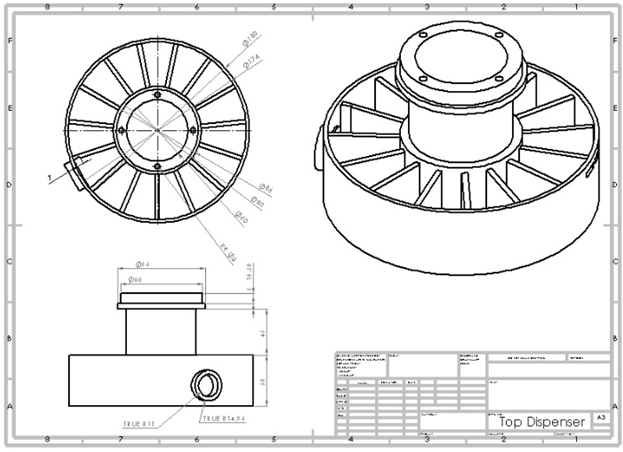
\includegraphics[width=1\linewidth]{A1.png}
	\caption{Top Dispenser Drawing}
\end{figure}
\newpage
\section{Bios}
\gadd{
\subsection{Chongdan Pan}
\begin{figure}[H]
    \centering
    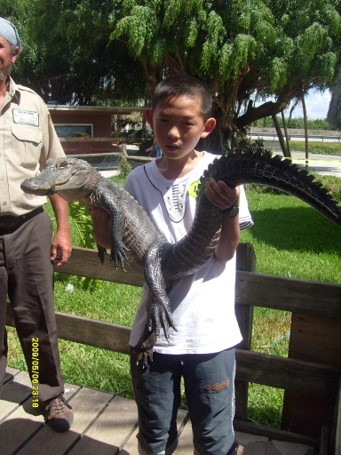
\includegraphics[width=2in]{p.jpg}
    \caption{Chongdan Pan}
    \label{fig::pan}
\end{figure}
Pan, Chongdan is a senior student major in electronic and computer engineering. He has gathered some experience in robotic field by participating a few robotic competitions. He has won an Asia champion and world champion in VEX robotic championship, and he will continue to study robots in the future. Now, he is applying for graduate programs related in computer engineering and robotics in the United States. In our project, he is mainly responsible for overall design and providing sources like tutorial or 3D print.
\subsection{Fernando Boaro}
\begin{figure}[H]
    \centering
    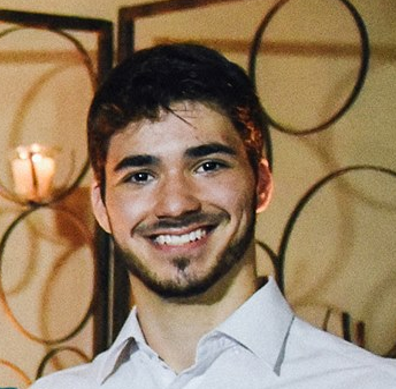
\includegraphics[width=2in]{f.png}
    \caption{Fernando Boaro}
    \label{fig::fer}
\end{figure}
Fernando Boaro is an undergraduate student completing his Mechanical Engineering studies in Shanghai Jiao Tong University, with an expected graduation on March, 2020. Fernando has completed two internships during his time at Jiao Tong, spending three months in Flieden, Germany as a mechanical engineering intern at A.I.C. RobotiX UG, a robotics startup company focusing on warehouse robots, where his main tasks were research and development and CAD design. And in 2019 completing another three month internship as a mechanical engineering intern at Mikron Industrial Automation in Shanghai, China, where his main tasks were the redesign of a protective machine door and designing CAD parts for customer projects. After his university studies Fernando plans to move to Germany and work as a mechanical engineer in the industrial robot industry.
\subsection{Niyiqiu Liu}
\begin{figure}[H]
    \centering
    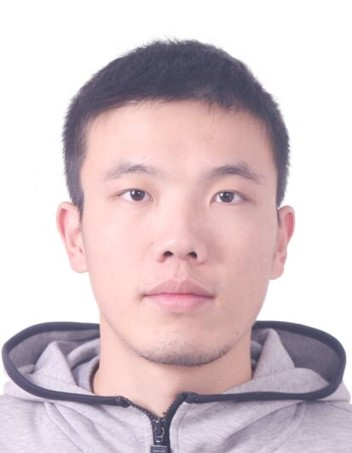
\includegraphics[width=2in]{l.jpg}
    \caption{Niyiqiu Liu}
    \label{fig::liu}
\end{figure}
Liu Niyiqiu is a senior student major in ECE. He is now following the computer science track in the ECE degree and is applying for graduate programs in the United States. He is in charge of software side of the project.
\subsection{Ruixing Zhou}
\begin{figure}[H]
    \centering
    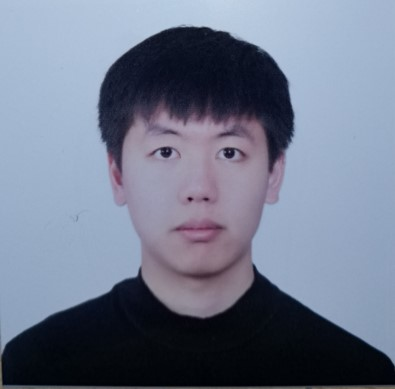
\includegraphics[width=2in]{z.jpg}
    \caption{Ruixing Zhou}
    \label{fig::zhou}
\end{figure}
Zhou Ruixing, a senior student major in ME, is focusing on the manufacturing area in the mechanical engineering degree. He has a good knowledge in engineering design and is well-experienced in CAD drawing. He is responsible for the structure design \& manufacture part of this project.
\subsection{Tianyu Qiu}
\begin{figure}[H]
    \centering
    
\includegraphics[width=2in]{q.jpg}
    \caption{Tianyu Qiu}
    \label{fig::qiu}
\end{figure}
Qiu Tianyu is a senior student major in ECE. He has great interest in circuit design and control system and is applying for graduate programs in the United States in Electrical Engineering. He is in charge of coding and circuit design in the project.}
\end{document}
